\documentclass[11pt]{article}  % need to compile twice
\usepackage{amsmath, textcomp, amssymb, geometry, graphicx, enumerate, ctex, float, multirow}
\usepackage[colorlinks, linkcolor=black]{hyperref}
\usepackage[table,xcdraw]{xcolor}

\geometry{left=2.54cm, right=2.54cm, top=3.18cm, bottom=3.18cm}

\def\Name{杨豪\space}  % Your name
\def\SID{2206213297}  % Your student ID number

%%%%%%%%%%%%%%%%%%%%%%%%%%%%%%%%%%%%%%%%%%%%%%%%%%%%%%%%%%%%%%
% need to be confirmed before each time writing and committing 
\def\Homework{4} % Number of Homework
\def\Session{2022-Fall}
\def\CourseCodeName{SOFT400127: Computer Organization \& Architecture}
\def\simCourseName{OA}

\title{\vspace{-4cm}\CourseCodeName \space
        \Session \protect\\  Homework-\textbf{\Homework} Solutions}
\author{软件2101 \Name \space 学号: \SID}
\markright{\simCourseName\ \space \Session\  HW-\Homework\ \Name}
\date{\today}



\begin{document}
\maketitle

\textbf{Honor Code: I promise that I finished the homework solutions on my own without copying other people's 
    work.}
    
\section*{1. } 
% Please add the following required packages to your document preamble:
% \usepackage[table,xcdraw]{xcolor}
% If you use beamer only pass "xcolor=table" option, i.e. \documentclass[xcolor=table]{beamer}
\begin{table}[H]
    \centering
    \begin{tabular}{|>{\columncolor[HTML]{FFFFFF}}c >{\columncolor[HTML]{FFFFFF}}c |}
        \hline
        \multicolumn{1}{|c|}{\cellcolor[HTML]{FFFFFF}{\color[HTML]{273239} \textbf{SRAM}}}                                                                        & {\color[HTML]{273239} \textbf{DRAM}}                                                                                                                        \\ \hline
        \multicolumn{2}{|c|}{\cellcolor[HTML]{FFFFFF}{\color[HTML]{273239} Power needed to preserve data}}                                                                                                                                                                                                                      \\ \hline
        \multicolumn{1}{|c|}{\cellcolor[HTML]{FFFFFF}{\color[HTML]{273239} use transistors to store information.}}                                                & {\color[HTML]{273239} use capacitors store information.}                                                                                                    \\ \hline
        \multicolumn{1}{|c|}{\cellcolor[HTML]{FFFFFF}{\color[HTML]{273239} \begin{tabular}[c]{@{}c@{}}no refreshing is required.\\ (No capacitors)\end{tabular}}} & {\color[HTML]{273239} \begin{tabular}[c]{@{}c@{}}capacitors need to be refreshed periodically\\ to store data for a long time.\end{tabular}} \\ \hline
        \multicolumn{1}{|c|}{\cellcolor[HTML]{FFFFFF}{\color[HTML]{273239} faster}}                                                                               & {\color[HTML]{273239} slower access speeds.}                                                                                                                \\ \hline
        \multicolumn{1}{|c|}{\cellcolor[HTML]{FFFFFF}{\color[HTML]{273239} no refreshing unit, smaller memory unit}}                                              & {\color[HTML]{273239} need refreshing unit, bigger memory unit.}                                                                                            \\ \hline
        \multicolumn{1}{|c|}{\cellcolor[HTML]{FFFFFF}{\color[HTML]{273239} more expensive}}                                                                       & {\color[HTML]{273239} cheaper}                                                                                                                              \\ \hline
        \multicolumn{1}{|c|}{\cellcolor[HTML]{FFFFFF}{\color[HTML]{273239} low-density devices}}                                                                  & {\color[HTML]{273239} high-density devices}                                                                                                                 \\ \hline
        \multicolumn{1}{|c|}{\cellcolor[HTML]{FFFFFF}{\color[HTML]{273239} In this bits are stored in voltage form.}}                                             & {\color[HTML]{273239} In this bits are stored in the form of electric energy.}                                                                              \\ \hline
        \multicolumn{1}{|c|}{\cellcolor[HTML]{FFFFFF}{\color[HTML]{273239} used in cache memories}}                                                               & {\color[HTML]{273239} used in main memories}                                                                                                                \\ \hline
        \multicolumn{1}{|c|}{\cellcolor[HTML]{FFFFFF}{\color[HTML]{273239} less power}}                                                                           & {\color[HTML]{273239} more power}                                                                                                                           \\ \hline
    \end{tabular}
\end{table}

\section*{2. }
Idea: Use memory hierarchy between main memory and cache —— multi-level caches.
Hardware Technology: 
\begin{itemize}
    \item Enhanced DRAM: Contains small SRAM as well SRAM holds last line read.
    \item Cache DRAM: Larger SRAM component and used as cache or serial buffer.
    \item Synchronous DRAM (SDRAM): 
    Access is synchronized with an external clock, so CPU knows when data will be ready.
    Also, data can be loaded with burst mode.
    As a result, CPU does not have to wait but can do something else.
    \begin{itemize}
        \item DDR SDRAM: Double-data-rate SDRAM can send data twice instead once per clock cycle using both rising edge and falling edge.
    \end{itemize}
\end{itemize}

\section*{3. }

\subsection*{3.1}

Answer:  $2^{22}\times \dfrac{32~\text{bits}}{8~\text{bits per byte}} = 4~\text{M} \times 4~\text{B} = \textbf{16 MB}$

\subsection*{3.2}

Answer: $\dfrac{16~\text{MB}}{512\times 2^{10} \times  16 / 8~\text{bytes}} = 16$ pieces.

\subsection*{3.3}

\begin{figure}[H]
    \centering
    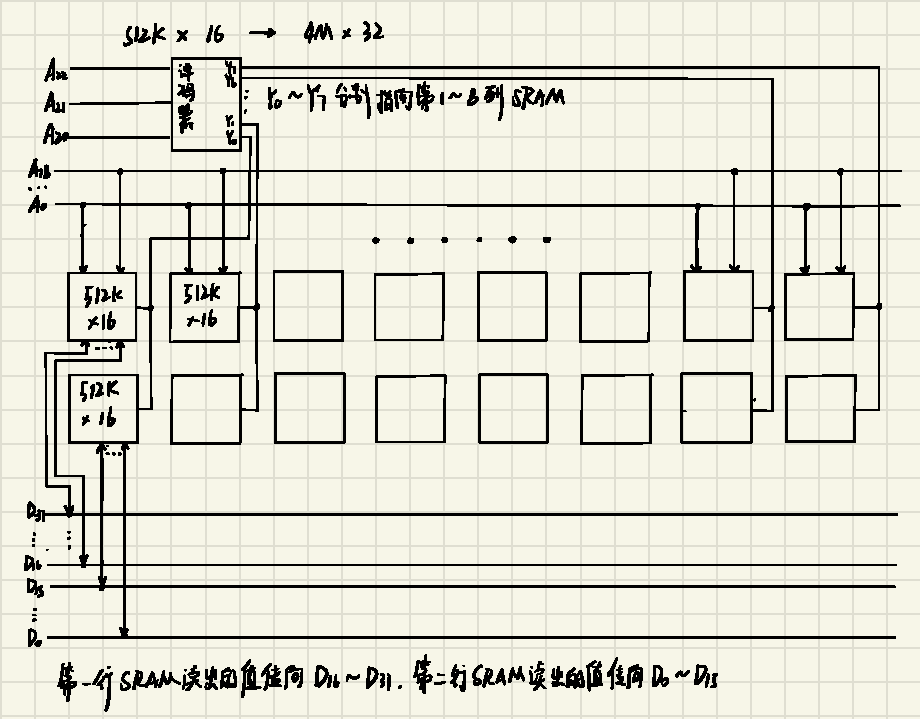
\includegraphics[width = 1\textwidth]{pic/2.pdf}
\end{figure}

\section*{4. }

\subsection*{Step 1\&2: Memory Capacity and Chip Section}
$\dfrac{8~\text{KB}}{4~\text{K}\times 8 / 8~\text{B}} = 2$, so choose two $~4~\text{K}\times8$ chips.

\subsection*{Step 3: Allocate CPU address lines}
$A_0-A_{11}$ to choose word inside a chip. Left high bits and MREQ are used for chip selection.
% Please add the following required packages to your document preamble:
\begin{table}[H]
    \centering
    \begin{tabular}{|l|c|c|ccc|c|c|c|}
    \hline
                           & Input & A15 & \multicolumn{3}{c|}{A14-A12}                        & A11 & …… & A0 \\ \hline
    \multirow{2}{*}{Chip1} & a000  & 1   & \multicolumn{1}{c|}{0} & \multicolumn{1}{c|}{1} & 0 & 0   & …… & 0  \\ \cline{2-9} 
                           & aFFF  & 1   & \multicolumn{1}{c|}{0} & \multicolumn{1}{c|}{1} & 0 & 1   & …… & 1  \\ \hline
    \multirow{2}{*}{Chip2} & b000  & 1   & \multicolumn{1}{c|}{0} & \multicolumn{1}{c|}{1} & 1 & 0   & …… & 0  \\ \cline{2-9} 
                           & bFFF  & 1   & \multicolumn{1}{c|}{0} & \multicolumn{1}{c|}{1} & 1 & 1   & …… & 1  \\ \hline
    \end{tabular}
\end{table}

\subsection*{Step 4: Draw the picture}

\begin{figure}[H]
    \centering
    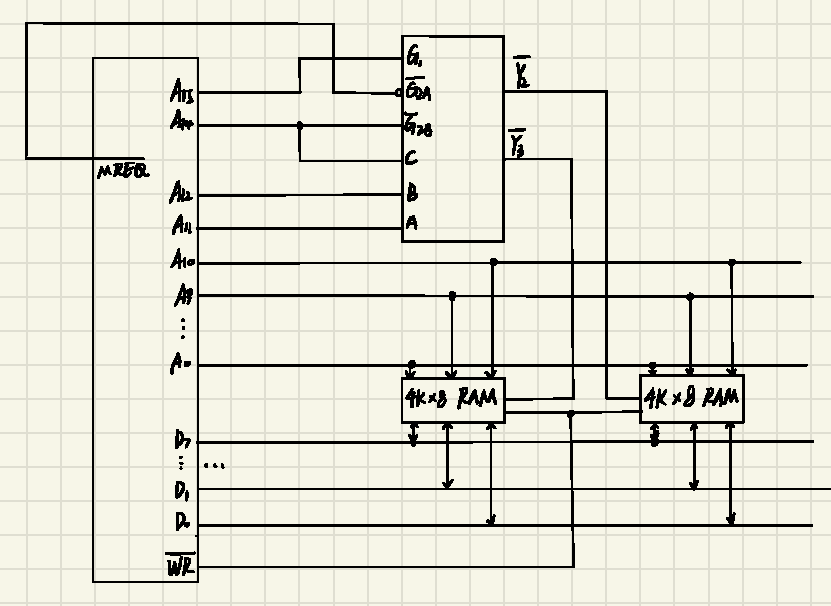
\includegraphics[width = 0.95\textwidth]{pic/1.pdf}
\end{figure}


\section*{Other things}

\begin{itemize}
    \item \LaTeX \space code refer to these things and was complied on texlive2020. 
    \begin{itemize}
        \item  \href{https://www.eecs70.org/assets/misc/homework_template.tex}{UCB-CS70's given homework template.} 
        \item  \href{https://www.latexlive.com}{A free website useful to edit \LaTeX \space formula code.}
    \end{itemize}
    \item refer to Professor Li.'s PPT.
\end{itemize}
%% The purpose of writing in English is to adapt to bilingual teaching and to improve my poor English 
%% writing skills in preparation for a possible future exchange program. 

    Thanks for your correcting and grading :).

\end{document}